\section{Conceptes}
\subsection{Motor de videojocs}
Un motor de videojocs és un conjunt d'eines i entorns de desenvolupament que faciliten la creació d'un videojoc. La definició és bastant oberta, ja que podem considerar com a motor des de un conjunt de llibreries independents, com és el cas amb Amethyst, fins a motors amb entorns gràfics d'alta complexitat com Unreal o Unity.

\subsection{Vòxels}
Podem definir un vòxel com la extensió al espai 3D d'un píxel. Dit d'altra manera, un vòxel és una sola casella dins d'una malla tridimensional. Si bé ja es feien servir freqüentment en anàlisi de dades mèdiques i científiques, en l'última dècada s'ha popularitzat el seu ús en videojocs, principalment gràcies a Minecraft.
\\
En comparació a mètodes més tradicionals per representar terreny, els vòxels faciliten la subdivisió del espai en trossos més petits, així com la manipulació i edició del terreny en temps real. A més, la simplicitat de la seva representació facilita molt el procés de carregar i desar conjunts de vòxels al emmagatzematge.
\subsection{Renderització}
S'anomena renderització al procés de convertir dades a imatges a través d'un programa informàtic. És un terme molt general, que pot descriure el procés de crear un video a través de software d'edició de video, o la representació en temps real d'un videojoc gràfic.
\subsection{Astrodinàmica}
L'atrodinàmica és el camp de la física que estudia el moviment dels cossos celestes no propulsats. Ja que el nostre objectiu és fer un videojoc en temps real, el que farem per simular les òrbites entre diversos cossos celestials serà integrar a partir de les següents fòrmules:
\begin{itemize}
  \item L'equació de gravitació universal de Newton, de forma $F=G\frac{m_{1}m_{2}}{r²}$ on $F$ és la força resultant, $G$ és la constant de gravitació universal, $m_{1}$ i $m_{2}$ són les masses dels dos cossos, i $r$ és la distància entre ells
  \item La segona llei de Newton, $F=ma$, on $F$ és la força, $m$ és la massa del cos, i $a$ és l'acceleració del cos.
\end{itemize}

\subsection{Entity Component System}
Entity component system és un patró de disseny de software utilitzat en el desenvolupament de videojocs. El patró especifica un sistema on tots els objectes del joc son una `entitat'. Fent ús de composició, les entitats no són més que agrupacions de diversos components, i cada component és actualitzat de forma independent per el sistema del mateix tipus.
\\
Per exemple, podem imaginar el component Cos. Tota entitat que tingui un cos físic i hagi de poder co\lgem isionar amb altres entitats i nodes tindrà un component Cos, el qual serà tant sols una estructura que emmagatzemarà les propietats del cos.
Per altra banda tindrem el sistema corresponent als cossos, el qual a cada actualització s'encarregarà de detectar i solucionar les possibles co\lgem isions entre cossos.
\\
Aquest patró facilita la modularitat de les entitats, i ajuda en gran mesura a crear i manipular entitats de forma dinàmica, on un objecte qualsevol podria obtenir la habilitat de, per exemple, volar, tant sols afegint-li el component corresponent.

\subsection{Gradient de soroll}
Un gradient de soroll és una funció matemàtica que genera valors numèrics pseudo-aleatòris dins d'un cert rang a partir d'unes coordenades d'entrada. Aquest soroll no és directament pseudo-aleatòri com podria ser-ho el soroll blanc, sinó que és generat mitjançant interpolació entre valors pseudo-aleatòris.
Aquesta interpolació fa que els valors del soroll en una certa àrea estiguin interrelacionats, i resulta en un soroll suau i poc abrupte.
En la figura ~\ref{fignoisecomparison} podem veure la diferència entre aquests tipus de soroll.
\begin{figure}[h]
  \hfill
  \subfigure[Exemple de soroll blanc]{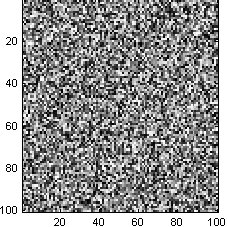
\includegraphics{whitenoise}}
  \hfill
  \subfigure[Exemple de gradient de soroll]{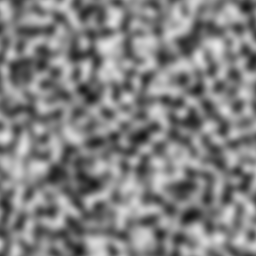
\includegraphics[scale=0.7]{coherentnoise}}
  \hfill
  \caption{Comparació de sorolls}
  \label{fignoisecomparison}
\end{figure}

\section{Termes}
A part dels conceptes explicats en aquest anterior apartat, en aquesta memòria farem servir alguns termes que s'expliquen a continuació.
\begin{itemize}
  \item{Node: }Anomenarem nodes als cossos astronòmics de la nostra simulació. Això engloba des del forat negre del centre de la via làctea amb un radi de $22\cdot10^{9}m$, fins a una petita nau espacial que el jugador ha construït dins del joc, amb unes dimensions de tant sols 10m³.
  \item{Entitat: }Anomenarem entitats a tots els personatges i objectes que interactuen amb el món. Exemples d'entitats podrien ser el pròpi jugador, un enemic, una pilota, o la càmera del joc.
\end{itemize}
